\begin{frame}
  \frametitle{\textbf{Jets}}
  \begin{columns}
    \column{0.5\textwidth}
    \begin{itemize}
    \item A jet is
      \begin{itemize}
      \item the result of a \textbf{high-}$\boldmath{Q^2}$ parton-parton interaction
      \item a \textbf{collimated spray of hadrons} resulting from parton fragmentation
      \item a \textbf{self-generating hard-probe} of the QGP
      \end{itemize}
    \item Jets are \textbf{well calibrated} in small systems (pp, $e^+ e^-$)
    \item Jets are often produced in back-to-back pairs
    \item $\tau^{\text{hard-scatter}} \ll \tau^{\text{QGP-formation}}$ $\to$ initial state unaffected by medium
    \item Use \textbf{relative jet yields} in pp and PbPb to measure medium properties
    \end{itemize}
    \column{0.5\textwidth}
    \centering 
    
    \begin{tikzpicture}
      \node{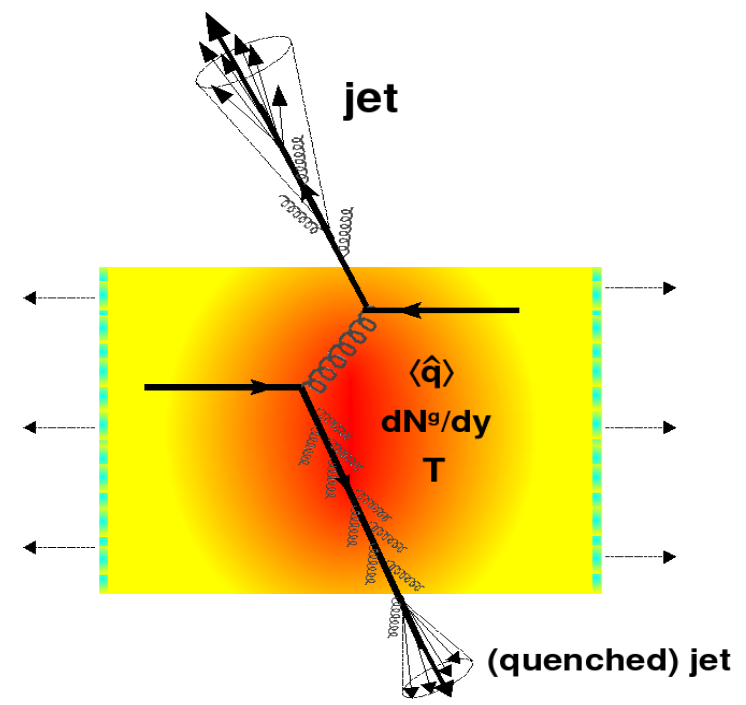
\includegraphics[width=0.8\textwidth]{jet-quenching.png}};
      \node[font=\tiny] at (1.5,1) {\href{https://arxiv.org/abs/0902.2011}{arXiv:0902.2011}};
    \end{tikzpicture}

    \

    \begin{tikzpicture}
      \node{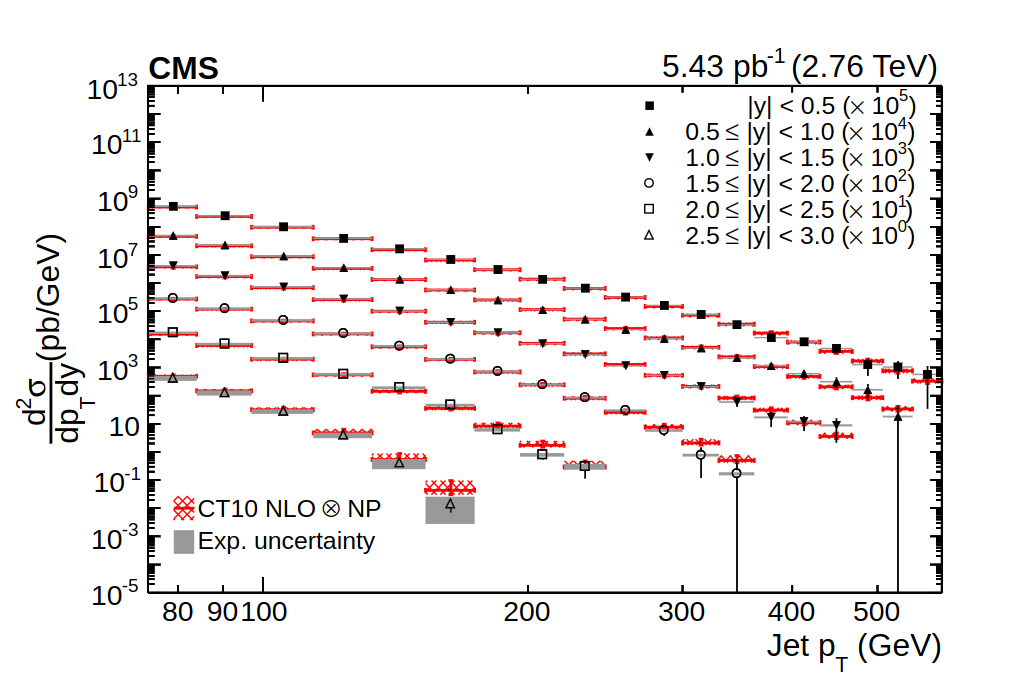
\includegraphics[width=0.8\textwidth]{jet-cross-section-data-vs-theory.png}};
      \node[font=\tiny] at (0.2,1.6) {\textbf{Jet production cross-section: data vs. theory}};
      \node[font=\tiny] at (-0.4,1.0) {\textbf{pp}};
      \node[font=\tiny] at (1.5,1) {\href{https://arxiv.org/abs/1512.06212}{arXiv:1512.06212}};
    \end{tikzpicture}


  \end{columns}







\end{frame}
